\iffalse
	\title{2017-XE-40-52}
	\author{EE24Btech11024 - G. Abhimanyu Koushik}
	\section{xe}
	\chapter{2017}
\fi

\item The Miller indices of the first three Bragg peaks in the X-ray diffraction pattern obtained from a polycrystalline iron sample at room temperature are

\hfill{\brak{\text{XE 2017}}}
\begin{enumerate}
\begin{multicols}{4}
\item \brak{111}, \brak{200}, \brak{220}
\item \brak{100}, \brak{110}, \brak{111}
\item \brak{100}, \brak{110}, \brak{200}
\item \brak{110}, \brak{200}, \brak{220}
\end{multicols}
\end{enumerate}

\item The number of close packed planes in the lattice of an FCC metal is

\hfill{\brak{\text{XE 2017}}}
\begin{enumerate}
\begin{multicols}{4}
\item 2
\item 4
\item 6
\item 12
\end{multicols}
\end{enumerate}

\item Which of the following treatment\brak{\text{s}} can increase the electrical conductivity of silicon?

\begin{enumerate}[label=(\roman*)]
    \item Heating
    \item Doping with arsenic
    \item Doping with aluminum
    \item Exposure to light
\end{enumerate}

\hfill{\brak{\text{XE 2017}}}
\begin{enumerate}
\begin{multicols}{2}
    \item Only \brak{\text{i}}
    \item Only \brak{\text{i}} and \brak{\text{ii}}
    \item Only \brak{\text{i}}, \brak{\text{ii}} and \brak{\text{iv}}
    \item All \brak{\text{i}}, \brak{\text{ii}}, \brak{\text{iii}} and \brak{\text{iv}}
\end{multicols}
\end{enumerate}

\item The unit cell volume of polyethylene \brak{\text{PE}} is $0.0933$ $nm^3$. Assuming two ethylene repeat units are contained within each unit cell, the density of a totally crystalline PE will be \rule{2.5cm}{0.4pt}$g/cm^3$. \lbrak{\text{Take the atomic weights for carbon and hydrogen as }12.01\text{ }g/mol\text{ and }1.008\text{ }g/mol\text{, respectively and }}\\ \rbrak{\text{Avagadro's number as }6.023\times 10^{23}\text{ repeat units/mol}}

\hfill{\brak{\text{XE 2017}}}

\item A continuous and aligned carbon fibre \brak{\text{CF}} reinforced polymer composite with $30\%$ of CF and rest resin was designed for a specific application. The modulus of elasticity of CF is $170$ $GPa$ and that of resin is $3.0$ $GPa$. The modulus of elasticity for this composite in the direction of fibre alignment is \rule{2.5cm}{0.4pt}$GPa$.

\hfill{\brak{\text{XE 2017}}}

\item Match the composites in Column $I$ with the most suitable application in Column $II$
\\\begin{table}[h!]    
  \centering
  \begin{tabular}{| p{6.5cm} | p{5cm} |}
\hline
\textbf{Column I} & \textbf{Column II} \\
\hline
P. Exfoliated silicates filled butyl rubber & 1. Automobile pistons \\
\hline
Q. Fibre reinforced aluminium alloy & 2. Contact lenses \\
\hline
R. Silicon carbide whiskers reinforced alumina & 3. Ski boards \\
\hline
S. Carbon particles reinforced plastic composites & 4. Tennis balls \\
\hline
& 5. Cutting tool inserts for machining \\
\hline
\end{tabular}
\end{table}\\

\hfill{\brak{\text{XE 2017}}}
\begin{enumerate}
\begin{multicols}{2}
\item P-$4$, Q-$1$, R-$5$, S-$3$
\item P-$2$, Q-$3$, R-$4$, S-$5$
\item P-$3$, Q-$5$, R-$5$, S-$3$
\item P-$2$, Q-$1$, R-$3$, S-$5$
\end{multicols}
\end{enumerate}

\item Match the processes in Column $I$ with products in Column $II$
\\\begin{table}[h!]    
  \centering
  \begin{tabular}{| p{4cm} | p{6cm} |}
    \hline
    \textbf{Column I} & \textbf{Column II} \\
    \hline
    P. Slip casting & 1. Metal powders \\
    \hline
    Q. Zone refining & 2. Thin films \\
    \hline
    R. Sputtering & 3. Ceramic parts \\
    \hline
    S. Atomization & 4. Single crystal \\
    \hline
    & 5. Metal sheets \\
    \hline
\end{tabular}
\end{table}\\

\hfill{\brak{\text{XE 2017}}}
\begin{enumerate}
\begin{multicols}{2}
\item P-$3$, Q-$4$, R-$2$, S-$1$
\item P-$2$, Q-$1$, R-$2$, S-$1$
\item P-$3$, Q-$4$, R-$5$, S-$1$
\item P-$3$, Q-$4$, R-$1$, S-$5$
\end{multicols}
\end{enumerate}

\item The value of diffusivity \brak{\text{D}} for the diffusion of carbon \brak{\text{C}} in $\gamma-$iron at $1300{{\degree}} C$ is \rule{2.5cm}{0.4pt}$\times 10^{-13}\text{ }m^2/s$. \brak{\text{Given }D_0=2\times 10^{-5}\text{ }m^2/s\text{; activation energy }Q=142\text{ }kJ/mol\text{; }R=8.314\text{ }J/mol\cdot K}

\hfill{\brak{\text{XE 2017}}}

\item Refer to the figure below:
\\\begin{center}
   \scalebox{0.5}{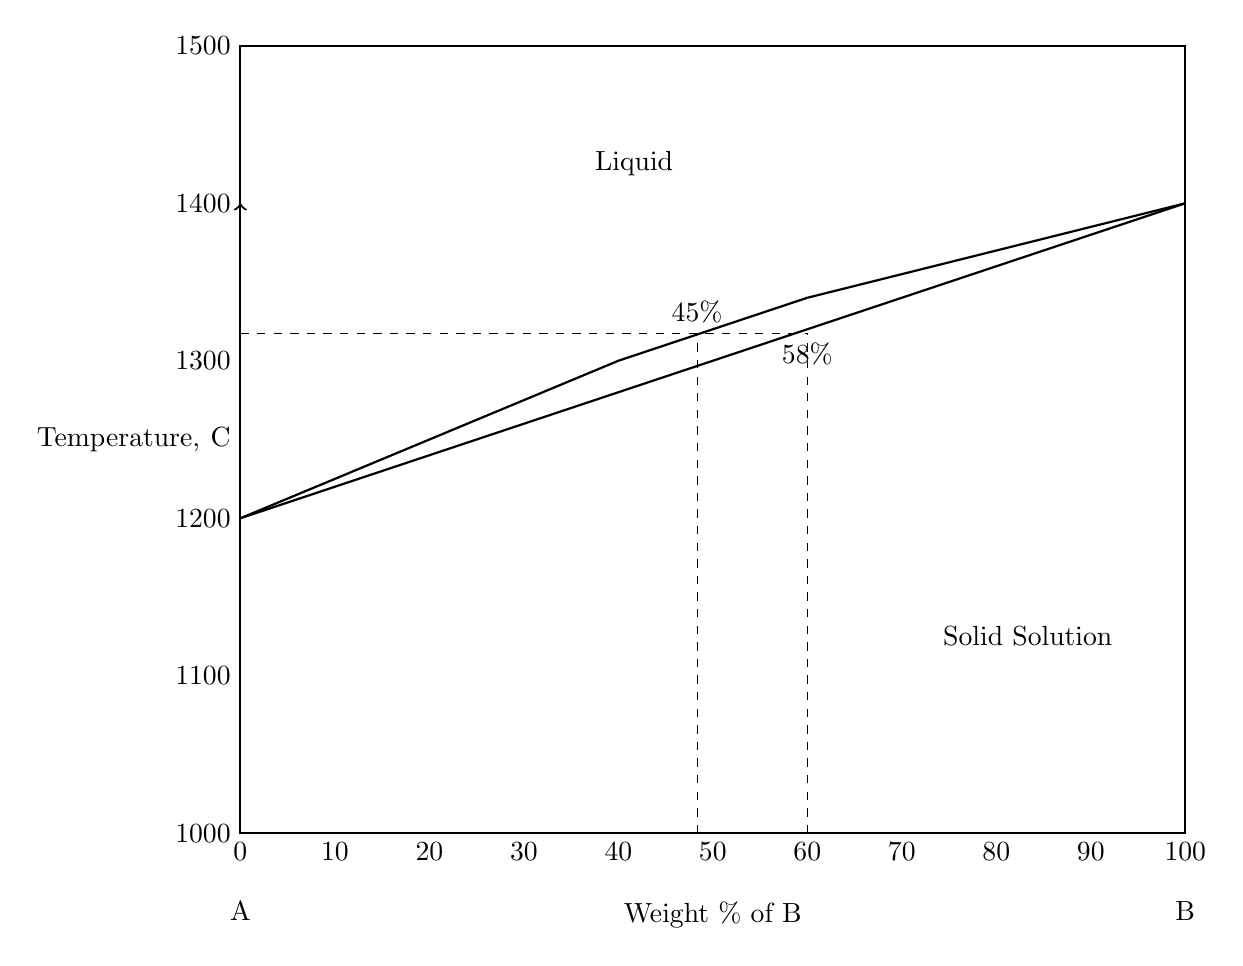
\begin{tikzpicture}

% Draw axes
\draw[thick,->] (0,0) rectangle (12,10);
\draw[thick,->] (0,0) -- (0,8);

% Add labels for the axes
\node[below] at (0,0) {0};
\node[below] at (1.2,0) {10};
\node[below] at (2.4,0) {20};
\node[below] at (3.6,0) {30};
\node[below] at (4.8,0) {40};
\node[below] at (6,0) {50};
\node[below] at (7.2,0) {60};
\node[below] at (8.4,0) {70};
\node[below] at (9.6,0) {80};
\node[below] at (10.8,0) {90};
\node[below] at (12,0) {100};
\node[left] at (0,0) {1000};
\node[left] at (0,2) {1100};
\node[left] at (0,4) {1200};
\node[left] at (0,6) {1300};
\node[left] at (0,8) {1400};
\node[left] at (0,10) {1500};

% Draw the phase lines
\draw[thick] (0,4) -- (4.8,6);
\draw[thick] (4.8,6) -- (7.2,6.8);
\draw[thick] (7.2,6.8) -- (12,8);
\draw[thick] (0,4) -- (12,8);

% Add dashed lines for composition percentages
\draw[dashed] (5.8,0) -- (5.8,6.35);
\draw[dashed] (7.2,0) -- (7.2,6.35);
\draw[dashed] (0,6.35) -- (7.2,6.35);

% Label the regions
\node[above] at (5.8,6.35) {45\%};
\node[below] at (7.2,6.35) {58\%};
\node at (5,8.5) {Liquid};
\node at (10,2.5) {Solid Solution};
\node[left] at (0,5) {Temperature, $^{{\degree}}$C};
\node[below] at (6,-0.75) {Weight $\%$ of B};
\node[below] at (0,-0.75) {A};
\node[below] at (12,-0.75) {B};

\end{tikzpicture}}
\end{center}
If the alloy contains $47$ wt. $\%$ of A and $53$ wt. $\%$ of B at $1300{{\degree}} C$, the wt. $\%$ of liquid present in the alloy at this temperature will be \rule{2.5cm}{0.4pt}

\hfill{\brak{\text{XE 2017}}}

\item Which of the following statement\brak{\text{s}} is/are true

\begin{enumerate}[label=(\roman*)]
    \item All piezoelectric materials are necessarily ferroelectric
    \item All ferroelectric materials are necessarily piezoelectric
    \item All pyroelectric materials are necessarily piezoelectric
    \item All pyroelectric materials are necessarily ferroelectric
\end{enumerate}

\hfill{\brak{\text{XE 2017}}}
\begin{enumerate}
\begin{multicols}{4}
    \item \brak{\text{i}} and \brak{\text{ii}}
    \item \brak{\text{ii}} and \brak{\text{iii}}
    \item \brak{\text{i}} and \brak{\text{iv}}
    \item \brak{\text{ii}} and \brak{\text{iv}}
\end{multicols}
\end{enumerate}


\item If the energy of formation of vacancies in pure copper is $0.9$ $eV$, the fraction of vacancies in pure copper at $27{{\degree}} C$ will be \rule{2.5cm}{0.4pt}$\times 10^{-16}$. \brak{\text{Boltzmann's constant is }8.62\times 10^{-5}\text{ }eV/K}

\hfill{\brak{\text{XE 2017}}}

\item A ceramic material with a critical flaw size of $30$ $\mu m$ has fracture stress of $300$ $MPa$. For the same material the fracture stress for a critical flaw size of $90$ $\mu m$ will be \rule{2.5cm}{0.4pt}$MPa$.

\hfill{\brak{\text{XE 2017}}}

\item An inorganic material that is transparent under solar light appears coloured when doped with transition metal ions. The possible reason\brak{\text{s}} for the colour is/are	

\begin{enumerate}[label=(\roman*)]
    \item The electronic energy levels of the host material changes significantly by doping
    \item The doped element selectively absorbs certain wavelength of light other than the perceived colour
    \item The doped element emits radiation of specific wavelength
\end{enumerate}

\hfill{\brak{\text{XE 2017}}}
\begin{enumerate}
\begin{multicols}{4}
    \item Only \brak{\text{i}}
    \item Both \brak{\text{i}} and \brak{\text{ii}}
    \item Both \brak{\text{i}} and \brak{\text{iii}}
    \item Both \brak{\text{ii}} and \brak{\text{iii}}
\end{multicols}
\end{enumerate}

